\documentclass[12pt, a4paper, oneside]{article}
\usepackage{arial}
\renewcommand{\familydefault}{\sfdefault}
\usepackage[T1]{fontenc}
\usepackage[polish]{babel}
\usepackage[utf8]{inputenc}
\usepackage{lmodern}
\usepackage[left=2cm,right=2cm,top=2cm,bottom=2cm]{geometry}
\selectlanguage{polish}
\usepackage{graphicx}
\usepackage{longtable}

\begin{document}
\section{Wykorzystane wzory}
Niepewność pomiaru rezystancji
\begin{equation}
u(R)=0.5\%~rdg+1~dgt
\end{equation}
Niepewność pomiaru indukcyjności
\begin{equation}
u(R)=3\%~rdg+10~dgt
\end{equation}
Wyznaczanie temperatury
\begin{equation}
T=\frac{R - 100}{0.392}+273.15
\end{equation}
Niepewność wyznaczonej temperatury
\begin{equation}
u_C(T)=|\frac{\partial T}{\partial R}\cdot u(R)|=\frac{u(R)}{0.392}
\end{equation}
Parametr $\frac{1}{\mu-1}$
\begin{equation}
\frac{1}{\mu-1}=\frac{1}{\frac{L}{L_0}-1}=\frac{T-T_C}{C}
\end{equation}
Niepewność wyznaczonego parametru $\frac{1}{\mu-1}$
\begin{equation}
u_C(\frac{1}{\mu-1})=|\frac{\partial \frac{1}{\frac{L}{L_0}-1}}{\partial L}\cdot u(L)|=\frac{L_0}{(L_0-L)^2\cdot u(L)}
\end{equation}
\section{Przykładowe obliczenia}
Niepewność pomiaru rezystancji
\begin{center}
$u(109.7)=0.005\cdot109.7+1\cdot 0.1=0.6485=0.65~[\Omega]$
\end{center}
Niepewność pomiaru indukcyjności
\begin{center}
$u(86.6)=0.03\cdot86.6+10\cdot 0.1=3.598=3.6~[mH]$
\end{center}
Wyznaczanie temperatury
\begin{center}
$T(109.7)=\frac{109.7-1}{0.392}+273.15=297.895~[K]$
\end{center}
Niepewność wyznaczonej temperatury
\begin{center}
$u_C(109.7)=\frac{0.65}{0.392}=1.6581=1.7~[K]$
\end{center}
Parametr $\frac{1}{\mu-1}$
\begin{center}
$\frac{1}{\mu-1}=\frac{1}{\frac{86.6}{42.5}-1}=0.96372$
\end{center}
Niepewność wyznaczonego parametru $\frac{1}{\mu-1}$
\begin{center}
$u_C(0.96372)=\frac{42.5}{(42.5-86.6)^2}\cdot 3.6=0.0786=0.079$
\end{center}
\clearpage
\section{Wyniki pomiarów i opracowanie}
\subsection{Chłodzenie układu}
% Table generated by Excel2LaTeX from sheet 'Arkusz1'
\begin{longtable}{|c|c|c|c|c|c|c|c|}
\caption{Wyniki pomiaru rezystancji oraz indukcyjności, wyznaczona temperatura oraz $\frac{1}{\mu-1}$, a także niepewności pomiarowe i złożone tych wartości}
\label{variability_impl_mech}
\endfirsthead
\endhead
\hline
    $R~[\Omega]$ & $u(R)~[\Omega]$ & $T~[K]$ & $u_C(T)~[K]$ & $L~[mH]$ & 
    $u(L)~[mH]$ & $\frac{1}{\mu-1}$ & $u_C(\frac{1}{\mu-1})$ \\\hline
    109.70 & 0.65 & 297.9 & 1.7 & 86.6 & 3.6 & 0.964 & 0.079 \\\hline
    109.60 & 0.65 & 297.6 & 1.7 & 86.7 & 3.7 & 0.962 & 0.081 \\\hline
    109.50 & 0.65 & 297.4 & 1.7 & 87.1 & 3.7 & 0.95 & 0.08 \\\hline
    109.40 & 0.65 & 297.1 & 1.7 & 87.7 & 3.7 & 0.940 & 0.077 \\\hline
    109.30 & 0.65 & 296.9 & 1.7 & 88.3 & 3.7 & 0.928 & 0.075 \\\hline
    109.20 & 0.65 & 296.6 & 1.7 & 89.0 & 3.7 & 0.914 & 0.073 \\\hline
    109.10 & 0.65 & 296.4 & 1.7 & 90.1 & 3.8 & 0.893 & 0.072 \\\hline
    109.00 & 0.65 & 296.1 & 1.7 & 90.7 & 3.8 & 0.88 & 0.07 \\\hline
    108.90 & 0.65 & 295.9 & 1.7 & 91.5 & 3.8 & 0.867 & 0.068 \\\hline
    108.80 & 0.65 & 295.6 & 1.7 & 92.7 & 3.8 & 0.847 & 0.065 \\\hline
    108.70 & 0.65 & 295.3 & 1.7 & 94.1 & 3.9 & 0.824 & 0.063 \\\hline
    108.60 & 0.65 & 295.1 & 1.7 & 95.5 & 3.9 & 0.80 & 0.06 \\\hline
    108.50 & 0.65 & 294.8 & 1.7 & 98 & 4 & 0.771 & 0.056 \\\hline
    108.40 & 0.65 & 294.6 & 1.7 & 100 & 4 & 0.740 & 0.052 \\\hline
    108.30 & 0.65 & 294.3 & 1.7 & 102.4 & 4.1 & 0.710 & 0.049 \\\hline
    108.20 & 0.65 & 294.1 & 1.7 & 104.6 & 4.2 & 0.684 & 0.047 \\\hline
    108.10 & 0.65 & 293.8 & 1.7 & 108.7 & 4.3 & 0.642 & 0.042 \\\hline
    108.00 & 0.64 & 293.6 & 1.7 & 112.4 & 4.4 & 0.608 & 0.039 \\\hline
    107.90 & 0.64 & 293.3 & 1.7 & 118.1 & 4.6 & 0.562 & 0.035 \\\hline
    107.80 & 0.64 & 293.0 & 1.7 & 121.3 & 4.7 & 0.539 & 0.033 \\\hline
    107.70 & 0.64 & 292.8 & 1.7 & 128.2 & 4.9 & 0.496 & 0.029 \\\hline
    107.60 & 0.64 & 292.5 & 1.7 & 136.8 & 5.2 & 0.451 & 0.025 \\\hline
    107.50 & 0.64 & 292.3 & 1.7 & 142.5 & 5.3 & 0.425 & 0.023 \\\hline
    107.40 & 0.64 & 292.0 & 1.7 & 152.4 & 5.6 & 0.39 & 0.02 \\\hline
    107.30 & 0.64 & 291.8 & 1.7 & 156.7 & 5.8 & 0.372 & 0.019 \\\hline
    107.20 & 0.64 & 291.5 & 1.7 & 161.9 & 5.9 & 0.356 & 0.018 \\\hline
    107.10 & 0.64 & 291.3 & 1.7 & 168.8 & 6.1 & 0.337 & 0.017 \\\hline
    107.00 & 0.64 & 291.0 & 1.7 & 175.9 & 6.3 & 0.319 & 0.016 \\\hline
    106.90 & 0.64 & 290.8 & 1.7 & 182.3 & 6.5 & 0.304 & 0.015 \\\hline
    106.80 & 0.64 & 290.5 & 1.7 & 188.2 & 6.7 & 0.292 & 0.014 \\\hline
    106.70 & 0.64 & 290.2 & 1.7 & 198 & 7 & 0.274 & 0.013 \\\hline
    106.60 & 0.64 & 290.0 & 1.7 & 203.1 & 7.1 & 0.265 & 0.012 \\\hline
    106.50 & 0.64 & 289.7 & 1.7 & 209.9 & 7.3 & 0.254 & 0.012 \\\hline
    106.40 & 0.64 & 289.5 & 1.7 & 214.8 & 7.5 & 0.247 & 0.011 \\\hline
    106.30 & 0.64 & 289.2 & 1.7 & 219.4 & 7.6 & 0.240 & 0.011 \\\hline
    106.20 & 0.64 & 289.0 & 1.7 & 224.3 & 7.8 & 0.234 & 0.011 \\\hline
    106.10 & 0.64 & 288.7 & 1.7 & 229.2 & 7.9 & 0.2276 & 0.0097 \\\hline
    106.00 & 0.63 & 288.5 & 1.7 & 233.5 & 8.1 & 0.2225 & 0.0095 \\\hline
    105.90 & 0.63 & 288.2 & 1.7 & 238.2 & 8.2 & 0.2172 & 0.0091 \\\hline
    105.80 & 0.63 & 287.9 & 1.7 & 241.4 & 8.3 & 0.214 & 0.009 \\\hline
    $R~[\Omega]$ & $u(R)~[\Omega]$ & $T~[K]$ & $u_C(T)~[K]$ & $L~[mH]$ & 
    $u(L)~[mH]$ & $\frac{1}{\mu-1}$ & $u_C(\frac{1}{\mu-1})$ \\\hline
    105.70 & 0.63 & 287.7 & 1.7 & 244.1 & 8.4 & 0.2108 & 0.0088 \\\hline
    105.60 & 0.63 & 287.4 & 1.7 & 247.6 & 8.5 & 0.2072 & 0.0086 \\\hline
    105.50 & 0.63 & 287.2 & 1.7 & 250.1 & 8.6 & 0.2047 & 0.0085 \\\hline
    105.40 & 0.63 & 286.9 & 1.7 & 252.4 & 8.6 & 0.2025 & 0.0083 \\\hline
    105.30 & 0.63 & 286.7 & 1.7 & 255.2 & 8.7 & 0.1998 & 0.0082 \\\hline
    105.20 & 0.63 & 286.4 & 1.7 & 257.8 & 8.8 & 0.1974 & 0.0081 \\\hline
    105.10 & 0.63 & 286.2 & 1.7 & 259.1 & 8.8 & 0.196 & 0.008 \\\hline
    105.00 & 0.63 & 285.9 & 1.7 & 262.2 & 8.9 & 0.1934 & 0.0079 \\\hline
    104.90 & 0.63 & 285.7 & 1.7 & 264 & 9 & 0.1920 & 0.0079 \\\hline
    104.80 & 0.63 & 285.4 & 1.7 & 265 & 9 & 0.1907 & 0.0077 \\\hline
    104.70 & 0.63 & 285.1 & 1.7 & 267.1 & 9.1 & 0.1892 & 0.0077 \\\hline
    104.60 & 0.63 & 284.9 & 1.7 & 268.0 & 9.1 & 0.1885 & 0.0077 \\\hline
    104.50 & 0.63 & 284.6 & 1.7 & 269.9 & 9.1 & 0.1869 & 0.0075 \\\hline
    104.40 & 0.63 & 284.4 & 1.7 & 271.5 & 9.2 & 0.1856 & 0.0075 \\\hline
    104.30 & 0.63 & 284.1 & 1.7 & 272.6 & 9.2 & 0.1847 & 0.0074 \\\hline
    104.20 & 0.63 & 283.9 & 1.7 & 274.1 & 9.3 & 0.1835 & 0.0074 \\\hline
    104.10 & 0.63 & 283.6 & 1.7 & 275.4 & 9.3 & 0.1825 & 0.0073 \\\hline
    104.00 & 0.62 & 283.4 & 1.6 & 276.5 & 9.3 & 0.1816 & 0.0073 \\\hline
\end{longtable}%
\begin{figure}[h]
\centering
\caption{Zależność $\frac{1}{\mu-1}$ w funkcji temperatury podczas chłodzenia układu}
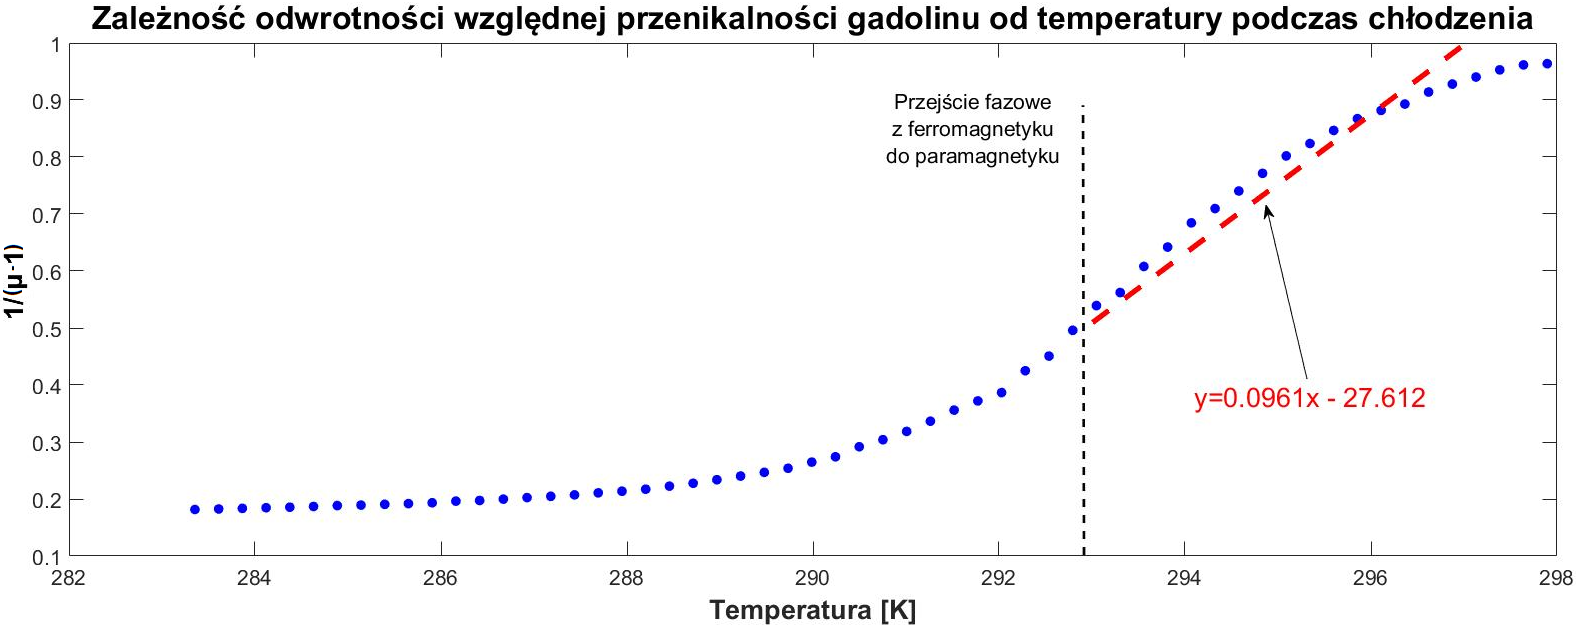
\includegraphics[scale=0.4]{f1.png}
\end{figure}
\indent	Dla części liniowej (po przejściu fazowym) wyznaczona została regresja liniowa, z wykorzystaniem funkcji REGLINP w programie Excel. Możemy z niej odczytać wartości współczynników $a$ oraz $b$. Stała Curie $C=\frac{1}{a}$, $u_C(C)=\frac{u(a)}{a^2}$ natomiast temperatura Curie $T_C=-\frac{b}{a}$, $u_C(T_C)=\sqrt{\frac{u^2(b)}{a^2}+\frac{b^2\cdot u^2(a)}{a^4}}$.\\

\noindent$C=(10.4 \pm 0.5)~K$\\
$T_C=(287\pm19)~K$
\clearpage
\subsection{Powrót układu do temperatury otoczenia (ogrzewanie)}
\begin{longtable}[h]{|c|c|c|c|c|c|c|c|}
\caption{Wyniki pomiaru rezystancji oraz indukcyjności, wyznaczona temperatura oraz $\frac{1}{\mu-1}$, a także niepewności pomiarowe i złożone tych wartości}
\label{variability_impl_mech}
\endfirsthead
\endhead
\hline
    $R~[\Omega]$ & $u(R)~[\Omega]$ & $T~[K]$ & $u_C(T)~[K]$ & $L~[mH]$ & 
    $u(L)~[mH]$ & $\frac{1}{\mu-1}$ & $u_C(\frac{1}{\mu-1})$ \\\hline
    104.00 & 0.62 & 283.4 & 1.6 & 276.5 & 9.3 & 0.1816 & 0.0073 \\\hline
    104.10 & 0.63 & 283.6 & 1.7 & 276.4 & 9.3 & 0.1817 & 0.0073 \\\hline
    104.20 & 0.63 & 283.9 & 1.7 & 275.9 & 9.3 & 0.1821 & 0.0073 \\\hline
    104.30 & 0.63 & 284.1 & 1.7 & 275.5 & 9.3 & 0.1824 & 0.0073 \\\hline
    104.40 & 0.63 & 284.4 & 1.7 & 274.8 & 9.3 & 0.1830 & 0.0074 \\\hline
    104.50 & 0.63 & 284.6 & 1.7 & 273.9 & 9.3 & 0.1837 & 0.0074 \\\hline
    104.60 & 0.63 & 284.9 & 1.7 & 273.0 & 9.2 & 0.1844 & 0.0074 \\\hline
    104.70 & 0.63 & 285.1 & 1.7 & 272.1 & 9.2 & 0.1851 & 0.0075 \\\hline
    104.80 & 0.63 & 285.4 & 1.7 & 270.5 & 9.2 & 0.1864 & 0.0076 \\\hline
    104.90 & 0.63 & 285.7 & 1.7 & 269.5 & 9.1 & 0.1872 & 0.0076 \\\hline
    105.00 & 0.63 & 285.9 & 1.7 & 268.7 & 9.1 & 0.1879 & 0.0076 \\\hline
    105.10 & 0.63 & 286.2 & 1.7 & 269.9 & 9.1 & 0.1869 & 0.0075 \\\hline
    105.20 & 0.63 & 286.4 & 1.7 & 266 & 9 & 0.1902 & 0.0077 \\\hline
    105.30 & 0.63 & 286.7 & 1.7 & 264 & 9 & 0.1923 & 0.0079 \\\hline
    105.40 & 0.63 & 286.9 & 1.7 & 261.8 & 8.9 & 0.1938 & 0.0079 \\\hline
    105.50 & 0.63 & 287.2 & 1.7 & 260.0 & 8.8 & 0.195 & 0.008 \\\hline
    105.60 & 0.63 & 287.4 & 1.7 & 257.4 & 8.8 & 0.1978 & 0.0081 \\\hline
    105.70 & 0.63 & 287.7 & 1.7 & 255.6 & 8.7 & 0.1994 & 0.0082 \\\hline
    105.80 & 0.63 & 287.9 & 1.7 & 254.0 & 8.7 & 0.2009 & 0.0083 \\\hline
    105.90 & 0.63 & 288.2 & 1.7 & 249.8 & 8.5 & 0.2050 & 0.0085 \\\hline
    106.00 & 0.63 & 288.5 & 1.7 & 247.1 & 8.5 & 0.2077 & 0.0087 \\\hline
    106.10 & 0.64 & 288.7 & 1.7 & 243.9 & 8.4 & 0.2110 & 0.0089 \\\hline
    106.20 & 0.64 & 289.0 & 1.7 & 240.8 & 8.3 & 0.214 & 0.009 \\\hline
    106.30 & 0.64 & 289.2 & 1.7 & 238.1 & 8.2 & 0.2173 & 0.0092 \\\hline
    106.40 & 0.64 & 289.5 & 1.7 & 234.9 & 8.1 & 0.2209 & 0.0093 \\\hline
    106.50 & 0.64 & 289.7 & 1.7 & 231 & 8 & 0.2252 & 0.0096 \\\hline
    106.60 & 0.64 & 290.0 & 1.7 & 227.1 & 7.9 & 0.2302 & 0.0099 \\\hline
    106.70 & 0.64 & 290.2 & 1.7 & 223.0 & 7.7 & 0.235 & 0.011 \\\hline
    106.80 & 0.64 & 290.5 & 1.7 & 220.5 & 7.7 & 0.239 & 0.011 \\\hline
    106.90 & 0.64 & 290.8 & 1.7 & 213.9 & 7.5 & 0.248 & 0.011 \\\hline
    107.00 & 0.64 & 291.0 & 1.7 & 208.4 & 7.3 & 0.256 & 0.012 \\\hline
    107.10 & 0.64 & 291.3 & 1.7 & 203.2 & 7.1 & 0.264 & 0.012 \\\hline
    107.20 & 0.64 & 291.5 & 1.7 & 195.8 & 6.9 & 0.277 & 0.013 \\\hline
    107.30 & 0.64 & 291.8 & 1.7 & 190.7 & 6.8 & 0.287 & 0.014 \\\hline
    107.40 & 0.64 & 292.0 & 1.7 & 182.2 & 6.5 & 0.304 & 0.015 \\\hline
    107.50 & 0.64 & 292.3 & 1.7 & 172.0 & 6.2 & 0.328 & 0.016 \\\hline
    107.60 & 0.64 & 292.5 & 1.7 & 162.2 & 5.9 & 0.355 & 0.018 \\\hline
    107.70 & 0.64 & 292.8 & 1.7 & 157.6 & 5.8 & 0.369 & 0.019 \\\hline
    107.80 & 0.64 & 293.0 & 1.7 & 145.8 & 5.4 & 0.411 & 0.022 \\\hline
    107.90 & 0.64 & 293.3 & 1.7 & 137.1 & 5.2 & 0.449 & 0.025 \\\hline
    108.00 & 0.64 & 293.6 & 1.7 & 132 & 5 & 0.474 & 0.027 \\\hline
    108.10 & 0.65 & 293.8 & 1.7 & 125.6 & 4.8 & 0.51 & 0.03 \\\hline
    $R~[\Omega]$ & $u(R)~[\Omega]$ & $T~[K]$ & $u_C(T)~[K]$ & $L~[mH]$ & 
    $u(L)~[mH]$ & $\frac{1}{\mu-1}$ & $u_C(\frac{1}{\mu-1})$ \\\hline
    108.20 & 0.65 & 294.1 & 1.7 & 118.5 & 4.6 & 0.559 & 0.034 \\\hline
    108.30 & 0.65 & 294.3 & 1.7 & 114.0 & 4.5 & 0.594 & 0.038 \\\hline
    108.40 & 0.65 & 294.6 & 1.7 & 109.9 & 4.3 & 0.631 & 0.041 \\\hline
    108.50 & 0.65 & 294.8 & 1.7 & 106.4 & 4.2 & 0.665 & 0.044 \\\hline
    108.60 & 0.65 & 295.1 & 1.7 & 103.5 & 4.2 & 0.697 & 0.048 \\\hline
    108.70 & 0.65 & 295.3 & 1.7 & 100.5 & 4.1 & 0.733 & 0.052 \\\hline
    108.80 & 0.65 & 295.6 & 1.7 & 98 & 4 & 0.767 & 0.056 \\\hline
    108.90 & 0.65 & 295.9 & 1.7 & 96.6 & 3.9 & 0.786 & 0.057 \\\hline
    109.00 & 0.65 & 296.1 & 1.7 & 94.5 & 3.9 & 0.817 & 0.062 \\\hline
    109.10 & 0.65 & 296.4 & 1.7 & 92.5 & 3.8 & 0.850 & 0.065 \\\hline
    109.20 & 0.65 & 296.6 & 1.7 & 91.4 & 3.8 & 0.869 & 0.068 \\\hline
    109.30 & 0.65 & 296.9 & 1.7 & 90.4 & 3.8 & 0.887 & 0.071 \\\hline
\end{longtable}
\begin{figure}[h]
\centering
\caption{Zależność $\frac{1}{\mu-1}$ w funkcji temperatury podczas powrotu do temperatury otoczenia}
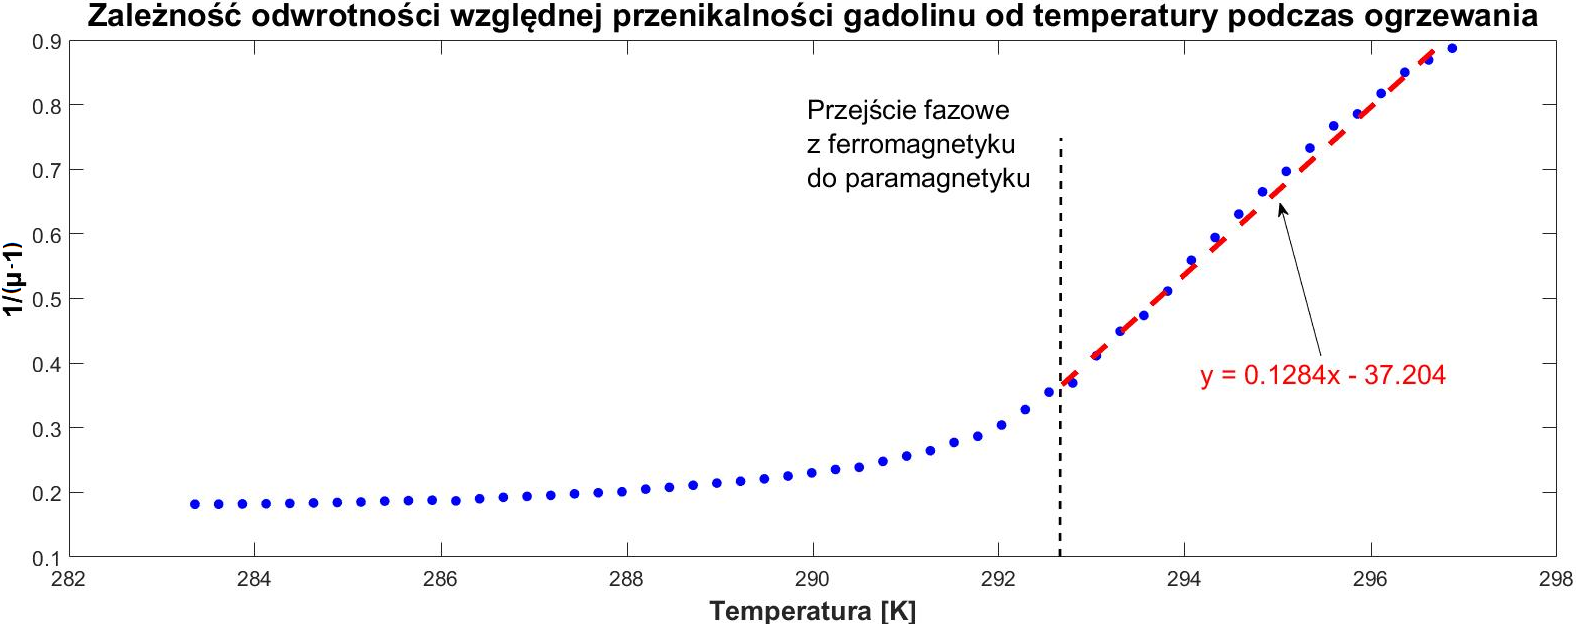
\includegraphics[scale=0.4]{f2.png}
\end{figure}
\indent	Dla części liniowej (po przejściu fazowym) wyznaczona została regresja liniowa, z wykorzystaniem funkcji REGLINP w programie Excel. Możemy z niej odczytać wartości współczynników $a$ oraz $b$. Stała Curie $C=\frac{1}{a}$, $u_C(C)=\frac{u(a)}{a^2}$ natomiast temperatura Curie $T_C=-\frac{b}{a}$, $u_C(T_C)=\sqrt{\frac{u^2(b)}{a^2}+\frac{b^2\cdot u^2(a)}{a^4}}$.\\

\noindent$C=(7.79 \pm 0.17)~K$\\
$T_C=(289\pm9)~K$
\subsection{Połączenie pomiarów}
Oba wykresy przedstawiają te same wartości, które częściowo są zbieżne, można je natomiast uśrednić dla uzyskania precyzyjniejszych wyników.\\

\noindent$\bar{C}=(9.09\pm0.27)~K$\\
$\bar{T_C}=(288\pm11)~K$
\clearpage
\section{Wnioski}
\begin{itemize}
\item Uzyskana z pomiarów stała Curie wynosi $\bar{C}=(9.09\pm0.27)~K$.
\item Uzyskana z pomiarów temperatura Curie wynosi $\bar{T_C}=(288\pm11)~K$.
\item Powyższe wartości wyznaczone zostały na podstawie uśrednienia wyników regresji liniowej dla pomiarów, podczas których układ był ochładzany, a następnie powracał do temperatury otoczenia.
\item Podczas ochładzania układu mogło zajść zbyt szybkie obniżanie temperatury, co z kolei prowadzi do mniej dokładnych wyników.
\item Dla odczytywanej wartości oporu, indukcyjność mieściła się w bardzo szerokim przedziale. Odczyt wykonywany był dla wartości oscylującej w okolicach środka przedziału.
\end{itemize}
\end{document}